\documentclass[11pt,a4paper]{article}
\usepackage[a4paper]{geometry}
\usepackage[utf8]{inputenc}
\usepackage[english]{babel}
\usepackage{lipsum}
\usepackage{eurosym}
\usepackage{rotating}

\usepackage{amsmath, amssymb, amsfonts, amsthm, mathtools}
% mathtools for: Aboxed (put box on last equation in align environment)
\usepackage{microtype} %improves the spacing between words and letters

% Packages for tables
\usepackage{threeparttable}
\usepackage{tabularx}
\usepackage{multirow}
\usepackage{booktabs}

\usepackage{lipsum}
\usepackage{threeparttable}
\usepackage{tabularx}
\usepackage{multirow}
\usepackage{booktabs}
\newcommand{\tabitem}{~~\llap{\textbullet}~~}
\usepackage{graphicx}
\graphicspath{ {./figures/} {./eps/}}
\usepackage{epsfig}
\usepackage{epstopdf}
\usepackage{verbatim}
\usepackage{textcomp}
\usepackage{tikz}
\usetikzlibrary{shapes,arrows}

\geometry{vmargin={2cm, 2cm}}
% Default fixed font does not support bold face
\DeclareFixedFont{\ttb}{T1}{txtt}{bx}{n}{12} % for bold
\DeclareFixedFont{\ttm}{T1}{txtt}{m}{n}{12}  % for normal

%%%%%%%%%%%%%%%%%%%%%%%%%%%%%%%%%%%%%%%%%%%%%%%%%%
%% COLOR DEFINITIONS
%%%%%%%%%%%%%%%%%%%%%%%%%%%%%%%%%%%%%%%%%%%%%%%%%%
 % Enabling mixing colors and color's call by 'svgnames'
%%%%%%%%%%%%%%%%%%%%%%%%%%%%%%%%%%%%%%%%%%%%%%%%%%
\definecolor{MyColor1}{HTML}{CC0000} %mix personal color
\newcommand{\textb}{\color{Black} \usefont{OT1}{lmss}{m}{n}}
\newcommand{\blue}{\color{MyColor1} \usefont{OT1}{lmss}{m}{n}}
\newcommand{\blueb}{\color{MyColor1} \usefont{OT1}{lmss}{b}{n}}
\newcommand{\red}{\color{LightCoral} \usefont{OT1}{lmss}{m}{n}}
\newcommand{\green}{\color{Turquoise} \usefont{OT1}{lmss}{m}{n}}
%%%%%%%%%%%%%%%%%%%%%%%%%%%%%%%%%%%%%%%%%%%%%%%%%%

%%%%%%%%%%%%%%%%%%%%%%%%%%%%%%%%%%%%%%%%%%%%%%%%%%
%% Scala coloring settings
%%%%%%%%%%%%%%%%%%%%%%%%%%%%%%%%%%%%%%%%%%%%%%%%%%
% "define" Scala
\usepackage{listings}
\usepackage{xcolor}
\lstset{escapeinside={<@}{@>}}
\definecolor{deepblue}{rgb}{0,0,0.5}
\definecolor{deepred}{rgb}{0.6,0,0}
\definecolor{deepgreen}{rgb}{0,0.5,0}

% Python style for highlighting
\newcommand\pythonstyle{\lstset{
language=Python,
basicstyle=\ttm,
otherkeywords={self},             % Add keywords here
keywordstyle=\ttb\color{deepblue},
emph={MyClass,__init__},          % Custom highlighting
emphstyle=\ttb\color{deepred},    % Custom highlighting style
stringstyle=\color{deepgreen},
frame=tb,                         % Any extra options here
showstringspaces=false            %
}}

% Python environment
\lstnewenvironment{python}[1][]
{
\pythonstyle
\lstset{#1}
}
{}

% Python for external files
\newcommand\pythonexternal[2][]{{
\pythonstyle
\lstinputlisting[#1]{#2}}}

% Python for inline
\newcommand\pythoninline[1]{{\pythonstyle\lstinline!#1!}}


%%%%%%%%%%%%%%%%%%%%%%%%%%%%%%%%%%%%%%%%%%%%%%%%%%
%% FONTS AND COLORS
%%%%%%%%%%%%%%%%%%%%%%%%%%%%%%%%%%%%%%%%%%%%%%%%%%
%		SECTIONS
%%%%%%%%%%%%%%%%%%%%%%%%%%%%%%%%%%%%%%%%%%%%%%%%%%
\usepackage{titlesec}
\usepackage{sectsty}
%%%%%%%%%%%%%%%%%%%%%%%%
%set section/subsections HEADINGS font and color
\sectionfont{\color{MyColor1}}  % sets colour of sections
\subsectionfont{\color{MyColor1}}  % sets colour of sections

%set section enumerator to arabic number (see footnotes markings alternatives)
\renewcommand\thesection{Exercise \arabic{section}} %define sections numbering
\renewcommand\thesubsection{\thesection.\arabic{subsection}} %subsec.num.

%define new section style
\newcommand{\mysection}{
\titleformat{\section} [runin] {\usefont{OT1}{lmss}{b}{n}\color{MyColor1}}
{\thesection} {3pt} {} }

%%%%%%%%%%%%%%%%%%%%%%%%%%%%%%%%%%%%%%%%%%%%%%%%%%
%		CAPTIONS
%%%%%%%%%%%%%%%%%%%%%%%%%%%%%%%%%%%%%%%%%%%%%%%%%%
\usepackage{caption}
\usepackage{subcaption}
%%%%%%%%%%%%%%%%%%%%%%%%
\captionsetup[figure]{labelfont={color=MyColor1}}

%%%%%%%%%%%%%%%%%%%%%%%%%%%%%%%%%%%%%%%%%%%%%%%%%%
%		!!!EQUATION (ARRAY) --> USING ALIGN INSTEAD
%%%%%%%%%%%%%%%%%%%%%%%%%%%%%%%%%%%%%%%%%%%%%%%%%%
%using amsmath package to redefine eq. numeration (1.1, 1.2, ...)
%%%%%%%%%%%%%%%%%%%%%%%%
\renewcommand{\theequation}{\arabic{equation}}

%set box background to grey in align environment
\usepackage{etoolbox}% http://ctan.org/pkg/etoolbox
\makeatletter
\patchcmd{\@Aboxed}{\boxed{#1#2}}{\colorbox{black!15}{$#1#2$}}{}{}%
\patchcmd{\@boxed}{\boxed{#1#2}}{\colorbox{black!15}{$#1#2$}}{}{}%
\makeatother
%%%%%%%%%%%%%%%%%%%%%%%%%%%%%%%%%%%%%%%%%%%%%%%%%%

\newcommand{\DP}[1]{\textcolor{blue}{\textbf{(DP says: #1)}}}

\makeatletter
\let\reftagform@=\tagform@
\def\tagform@#1{\maketag@@@{(\ignorespaces\textcolor{red}{#1}\unskip\@@italiccorr)}}
\renewcommand{\eqref}[1]{\textup{\reftagform@{\ref{#1}}}}
\makeatother
\usepackage[hidelinks]{hyperref}

%% LISTS CONFIGURATION %%
\usepackage{enumitem}
\setlist[enumerate,1]{start=0}
\renewcommand{\labelenumii}{\theenumii}
\renewcommand{\theenumii}{\theenumi.\arabic{enumii}.}

\usepackage[acronym]{glossaries}
\newacronym{ci}{CI}{Confidence Interval}
%%%%%%%%%%%%%%%%%%%%%%%%%%%%%%%%%%%%%%%%%%%%%%%%%%
%% PREPARE TITLE
%%%%%%%%%%%%%%%%%%%%%%%%%%%%%%%%%%%%%%%%%%%%%%%%%%
\title{\blue Network analysis and simulation\\ Homework 1}
\author{Davide Peron}
\date{}
%%%%%%%%%%%%%%%%%%%%%%%%%%%%%%%%%%%%%%%%%%%%%%%%%%

\begin{document}
\maketitle
\section{}
In the first exercise the implementation of a slotted queue is required.
The three different case follows:
\subsection{}
\label{ex:1.1}

\begin{figure}[ht]
\centering
\begin{subfigure}{.5\textwidth}
  \centering
  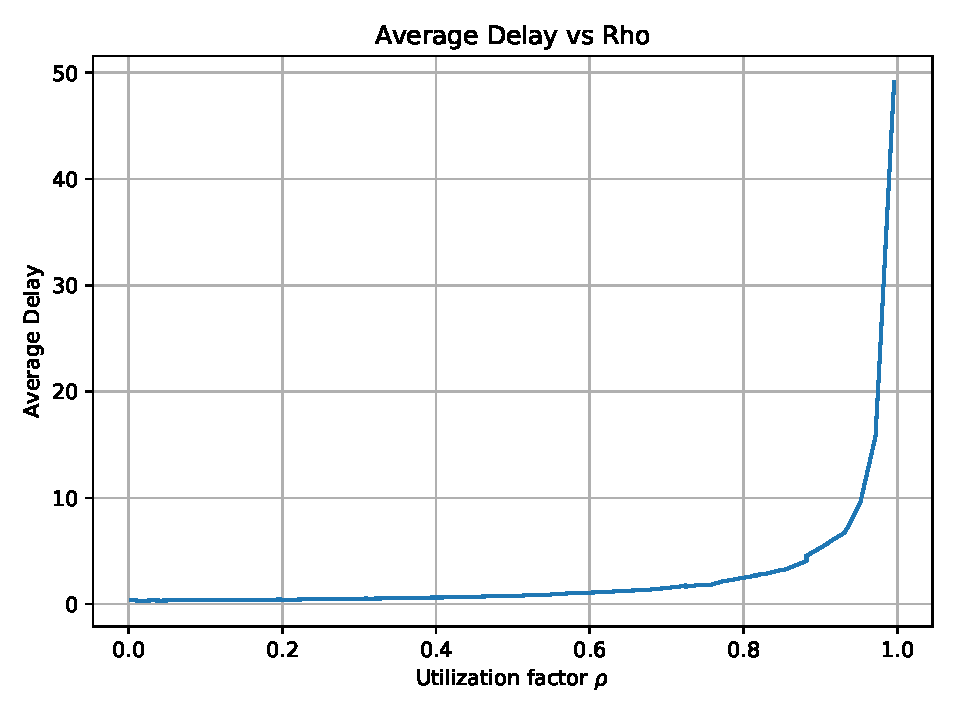
\includegraphics[width=\linewidth]{avg_delay_vs_rho_1}
  \caption{Average delay vs Utilization factor}
  \label{fig:delayRho1}
\end{subfigure}%
\begin{subfigure}{.5\textwidth}
  \centering
  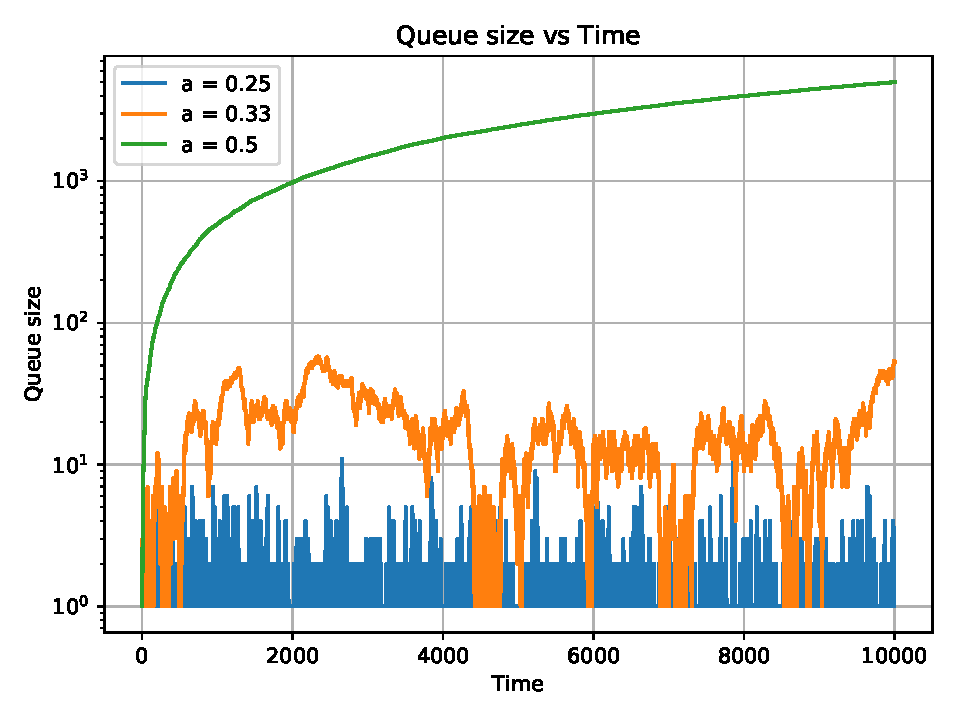
\includegraphics[width=\linewidth]{queue_size_vs_time_logy}
  \caption{Queue size vs time by varying $a$}
  \label{fig:queueSize1}
\end{subfigure}
\caption{Plots required in Exercise 1.1}
\end{figure}

In this first case is required to plot:
\begin{itemize}
\item the average delay in function of the utilization factor $\rho$ by varying $a$, that is the probability the 1 or 2 packets arrive to the queue, from 0 to 1/3, the result is in \autoref{fig:delayRho1}
\item a realization of the queue size in function of the time for 10000 slots for a = 1/4, 1/3 and 1/2, the result is in \autoref{fig:queueSize1}
\end{itemize}

From the second plot can be seen that for a = 1/2 the queue is unstable and its size diverges. Indeed from queueing theory we know that the arrival rate for this queue is:
\begin{equation}
  \lambda = 1 \cdot a + 2 \cdot a
\end{equation}
while the service time $\mu$ is one slot. To be stable, the queue has to satisfy \autoref{eq:stability1}, so, as simulated, in the first two cases the queue is stable.
\begin{equation}
  \label{eq:stability1}
  \lambda \le \mu \Rightarrow 3a \le 1 \Rightarrow a \le 1/3
\end{equation}

\subsection{}
\label{ex:1.2}

\begin{figure}[ht]
\centering
\begin{subfigure}{.5\textwidth}
  \centering
  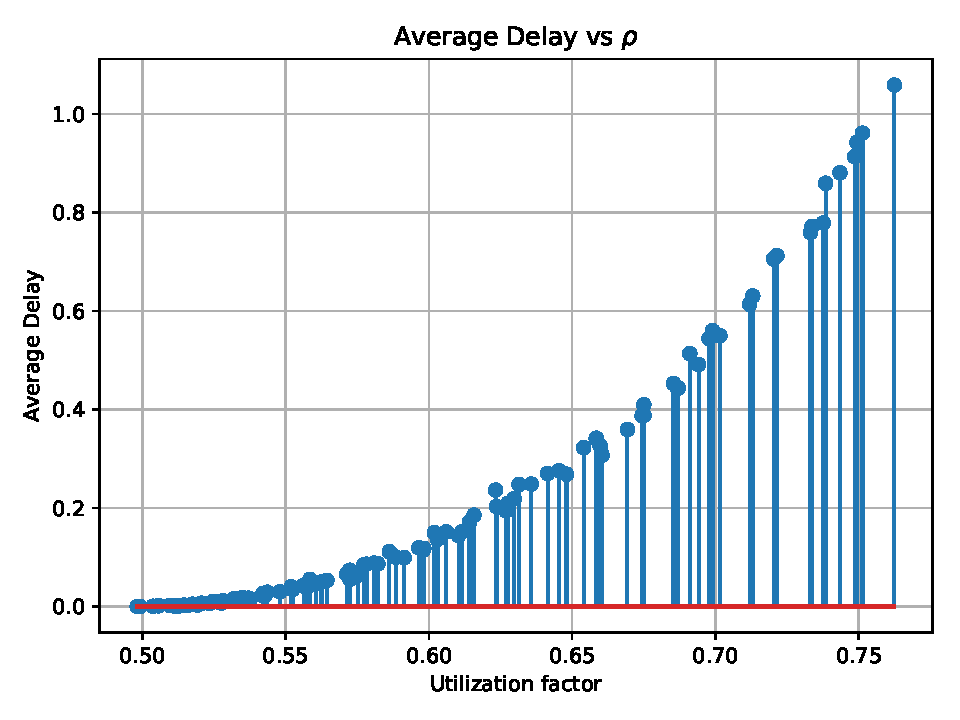
\includegraphics[width=\linewidth]{avg_delay_vs_rho_2}
  \caption{Average delay vs Utilization factor}
  \label{fig:delayRho2}
\end{subfigure}%
\begin{subfigure}{.5\textwidth}
  \centering
  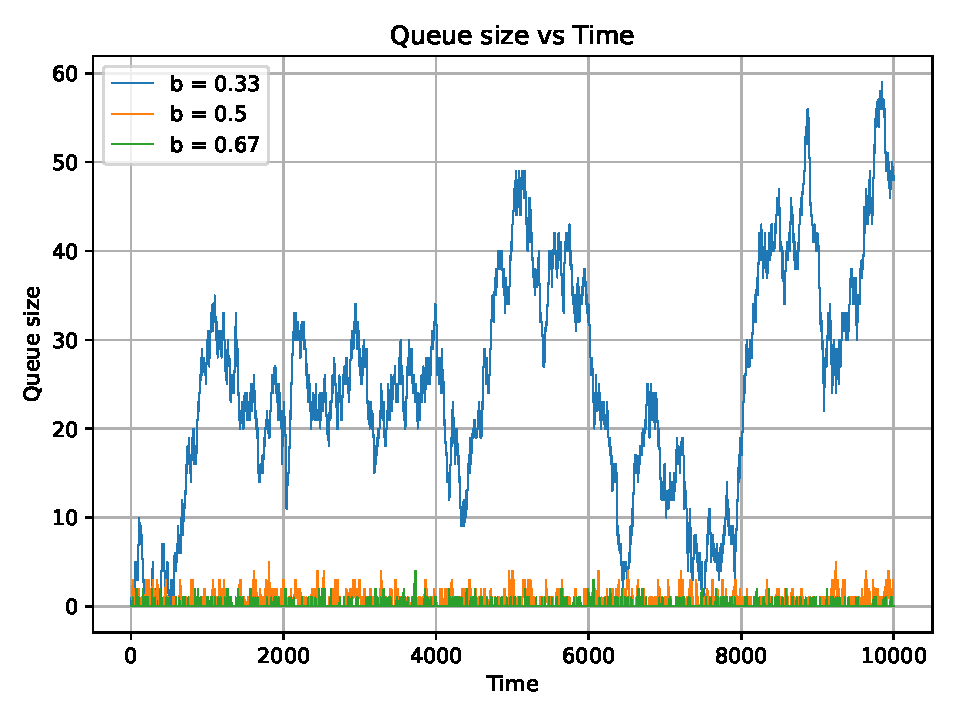
\includegraphics[width=\linewidth]{queue_size_vs_time_logy_es2}
  \caption{Queue size vs time by varying $b$}
  \label{fig:queueSize2}
\end{subfigure}
\caption{Plots required in Exercise 1.2}
\end{figure}
In the second case the same plots are required with the difference that this time the parameter to vary is b, i.e. the parameter of the geometric service time.

\subsection{}
In Exercise 1.1 the queue size for which $P[overflow]=0.00001$ is respectively 12 for $a=0.25$, 58 for $a=0.33$ and 61 for $a=0.5$ even if in the latter the queue is unstable, so eventually the queue will become full.

In Exercise 1.2 the queue size for which $P[overflow]=0.00001$ is respectively 81 for $b=0.33$, 9 for $b=0.5$ and 5 for $b=0.66$.
\newpage
\section{}
The second exercise is required to implement a raw simulator of a basic cellular network. In the follows the required plots are showed.

\begin{figure}[ht]
  \centering
  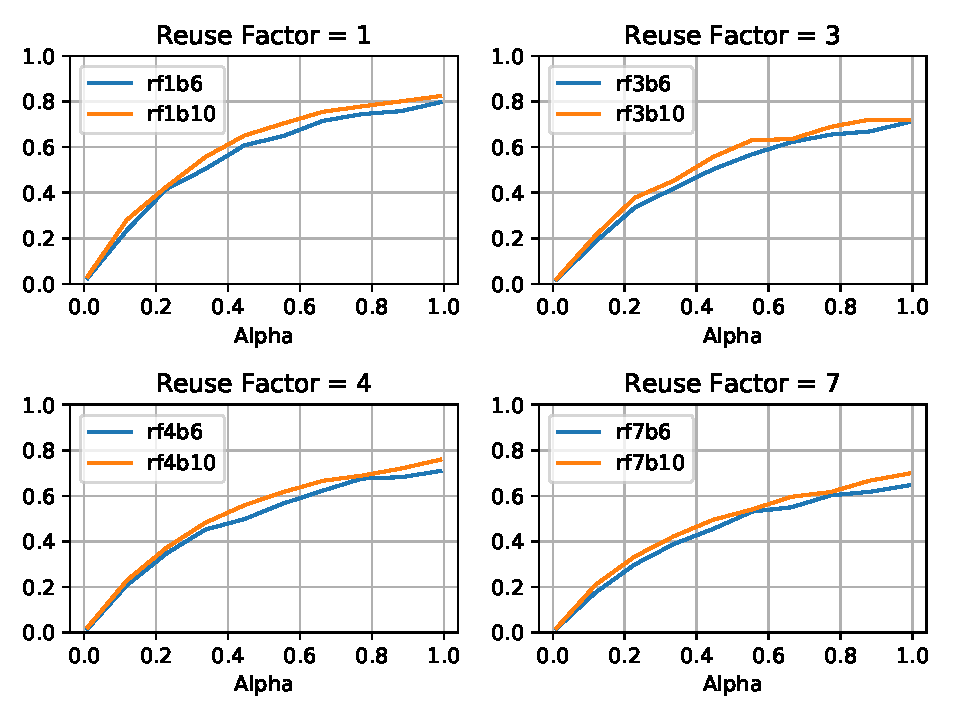
\includegraphics[width=\linewidth]{outage_montecarlo}
  \caption{Outage probabilities vs activity of interferers for six cells and reuse factor 1,3,4,7}
  \label{fig:outage}
\end{figure}

\section{}
The third exercise requires to perform a simulation study of the multihop performance of GeRaF using both Montecarlo simulations and numerical evaluation and to ripropose the figures showed in the paper.
The figures follows:

\begin{figure}[ht]
\centering
\begin{subfigure}{.45\textwidth}
  \centering
  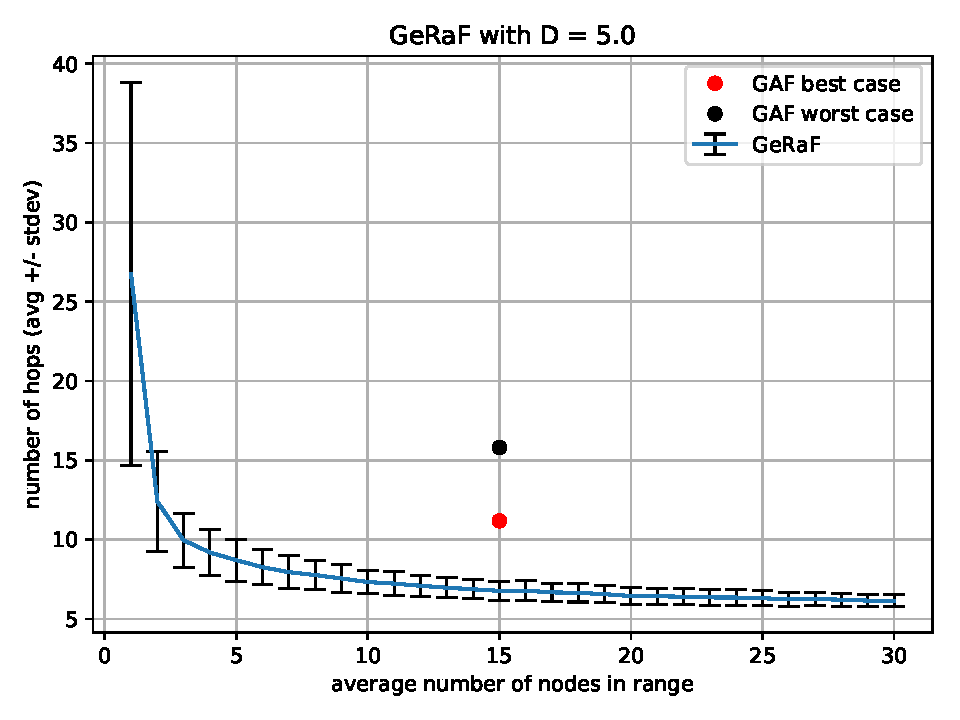
\includegraphics[width=\linewidth]{hops_montecarlo_D=5.pdf}
  \caption{Average number of hops $\pm$ standard deviation versus average number of active neighbors. Distance D = 5}
  \label{fig:hops5}
\end{subfigure}%
\hspace{0.5cm}
\begin{subfigure}{.45\textwidth}
  \centering
  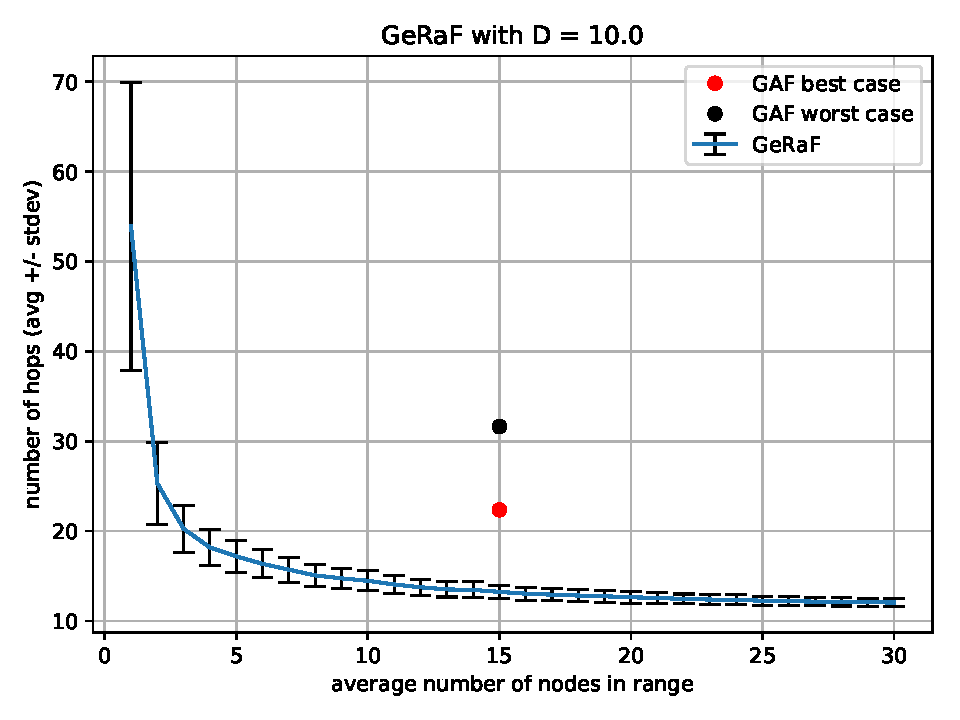
\includegraphics[width=\linewidth]{hops_montecarlo_D=10.pdf}
  \caption{Average number of hops $\pm$ standard deviation versus average number of active neighbors. Distance D = 10}
  \label{fig:hops10}
\end{subfigure}
\begin{subfigure}{.5\textwidth}
  \centering
  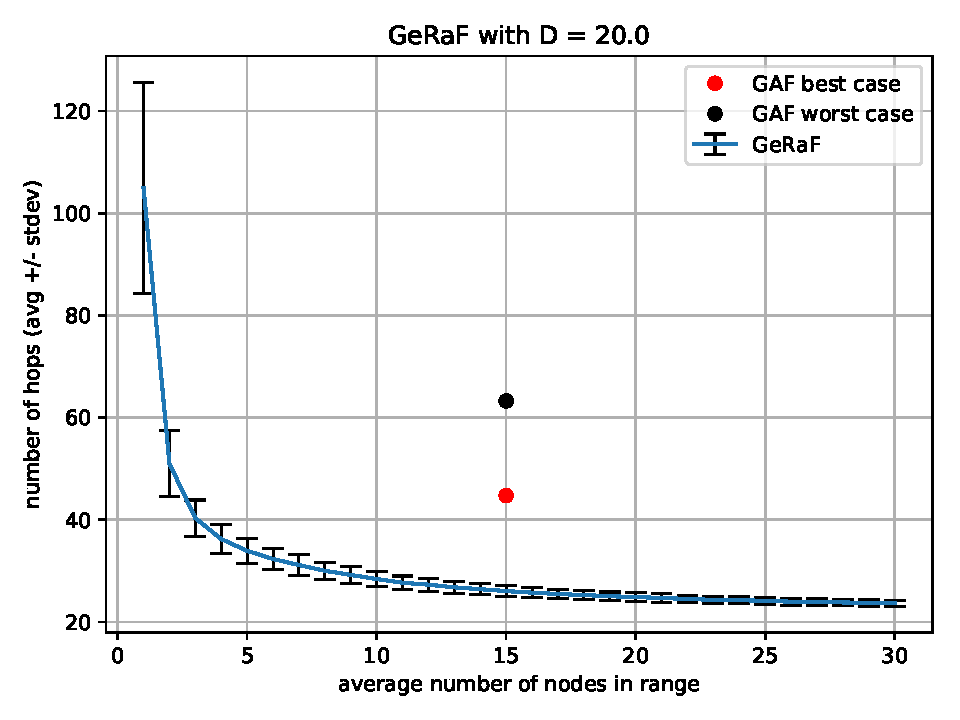
\includegraphics[width=\linewidth]{hops_montecarlo_D=20.pdf}
  \caption{Average number of hops $\pm$ standard deviation versus average number of active neighbors. Distance D = 20}
  \label{fig:hops20}
\end{subfigure}
\caption{Plots required in third exercise using Montecarlo simulations}
\end{figure}

\begin{figure}[ht]
\centering
\begin{subfigure}{.45\textwidth}
  \centering
  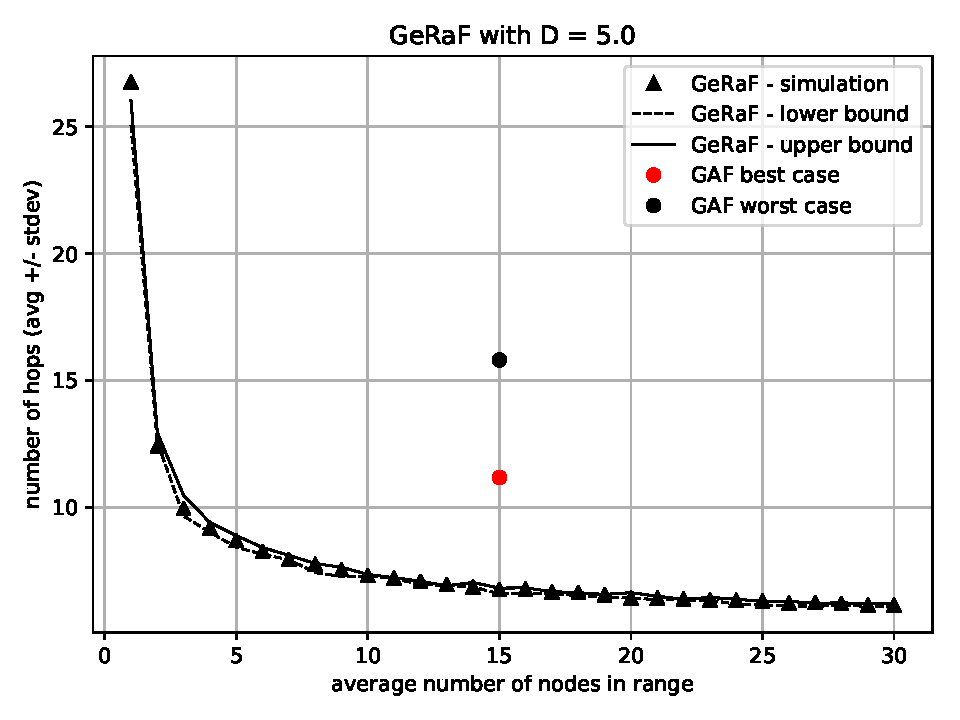
\includegraphics[width=\linewidth]{hops_bounds_D=5.pdf}
  \caption{Average number of hops $\pm$ standard deviation versus average number of active neighbors. Distance D = 5}
  \label{fig:hops5Bounds}
\end{subfigure}%
\hspace{0.5cm}
\begin{subfigure}{.45\textwidth}
  \centering
  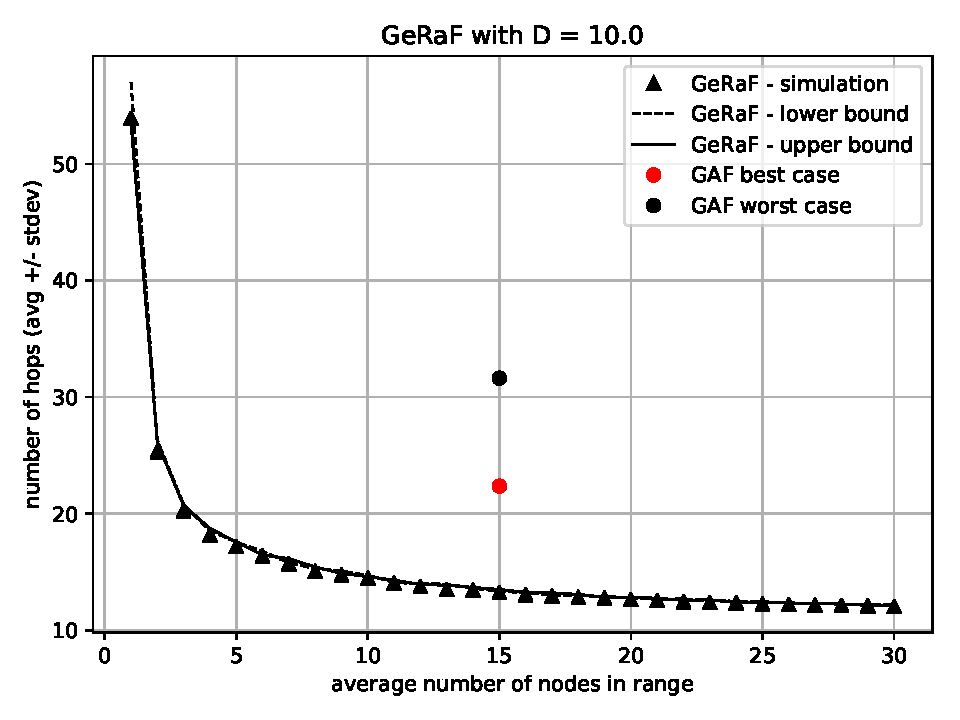
\includegraphics[width=\linewidth]{hops_bounds_D=10.pdf}
  \caption{Average number of hops $\pm$ standard deviation versus average number of active neighbors. Distance D = 10}
  \label{fig:hops10Bounds}
\end{subfigure}
\begin{subfigure}{.5\textwidth}
  \centering
  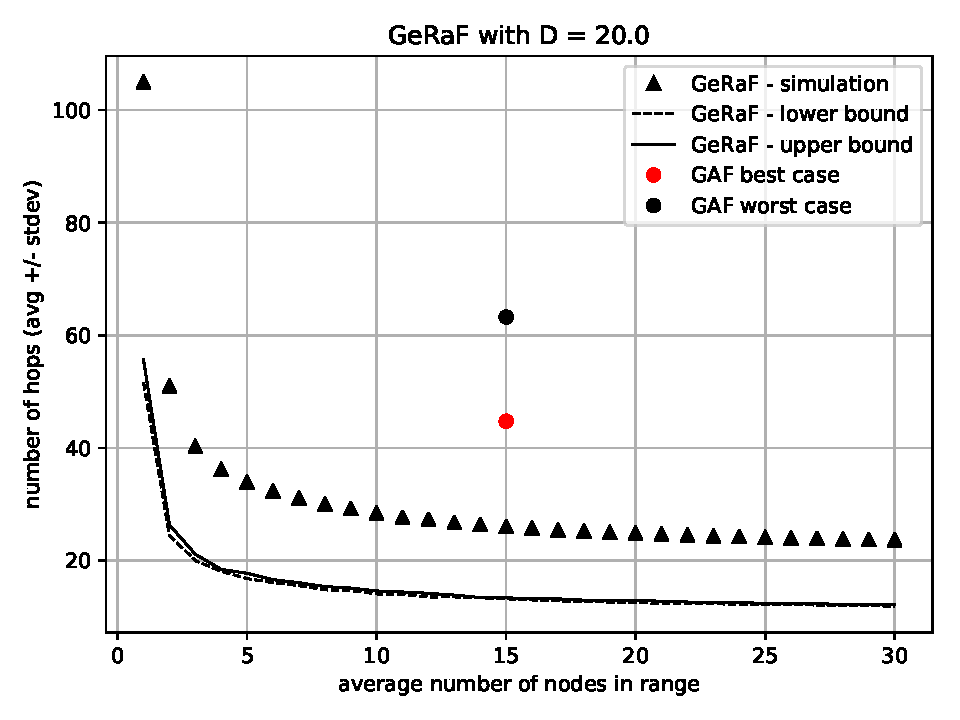
\includegraphics[width=\linewidth]{hops_bounds_D=20.pdf}
  \caption{Average number of hops $\pm$ standard deviation versus average number of active neighbors. Distance D = 20}
  \label{fig:hops20Bounds}
\end{subfigure}
\caption{Plots required in third exercise using numerical evaluation}
\end{figure}


\end{document}